\chapter{PROJECT MANAGEMENT PLAN}

\section{Giới thiệu chương}

Chương này trình bày kế hoạch quản lý dự án cho hệ thống \textbf{SEAL Hackathon Management System}. Kế hoạch được xây dựng nhằm xác định rõ phạm vi công việc, phương pháp tổ chức, cách phân công trách nhiệm, cơ chế theo dõi tiến độ, tiêu chuẩn chất lượng và phương thức quản lý mã nguồn trong suốt quá trình phát triển.

Dự án được thực hiện từ ngày \textbf{14/05/2026} đến ngày \textbf{12/07/2026}, với tổng thời gian 60 ngày nếu tính cả ngày bắt đầu và ngày kết thúc. Nhóm gồm năm thành viên, được phân công theo hai hướng chính là Frontend và Backend, đồng thời cùng tham gia vào các hoạt động phân tích yêu cầu, thiết kế, kiểm thử và viết báo cáo. Công việc được chia thành các Sprint kéo dài một tuần và theo dõi trên Jira. GitHub được sử dụng để quản lý mã nguồn, tài liệu kỹ thuật và báo cáo LaTeX. Các nhiệm vụ được đánh số theo mã dự án \texttt{N4SHM} và được theo dõi thông qua các trạng thái như \textit{To Do}, \textit{In Review} và \textit{Done}.

Nội dung của chương được tổ chức dựa trên cấu trúc của một Software Project Management Plan, bao gồm tổng quan phạm vi và ước lượng, mục tiêu dự án, quản lý rủi ro, phương pháp quản lý, kế hoạch chất lượng, sản phẩm bàn giao, phân công trách nhiệm, kế hoạch truyền thông và quản lý cấu hình.

\section{Tổng quan kế hoạch quản lý dự án}

\subsection{Phạm vi và ước lượng}

\subsubsection{Phạm vi của dự án}

\textbf{SEAL Hackathon Management System} là ứng dụng Web hỗ trợ quản lý các hoạt động cơ bản của một cuộc thi Hackathon. Phiên bản hiện tại tập trung vào quy trình dành cho thí sinh và đội thi, từ đăng ký tài khoản, đăng nhập, tạo đội, tham gia đội, quản lý thành viên cho đến nộp đường dẫn GitHub của sản phẩm dự thi.

Các chức năng nằm trong phạm vi triển khai bao gồm:

\begin{itemize}
    \item Đăng ký tài khoản bằng tên đăng nhập, email và mật khẩu.
    \item Đăng nhập hệ thống và xác thực người dùng bằng JWT Access Token.
    \item Tạo đội thi và tự động sinh mã mời gồm sáu ký tự.
    \item Gửi yêu cầu tham gia đội thông qua mã mời.
    \item Trưởng đội xem, phê duyệt hoặc từ chối yêu cầu tham gia.
    \item Xem danh sách thành viên chính thức của đội.
    \item Thành viên rời đội và trưởng đội loại thành viên khỏi đội.
    \item Trưởng đội giải tán đội khi cần thiết.
    \item Thành viên hợp lệ nộp hoặc cập nhật đường dẫn GitHub của bài dự thi.
    \item Hiển thị Dashboard theo trạng thái đội của người dùng.
    \item Xây dựng giao diện và API nguyên mẫu cho vai trò Judge và Admin.
\end{itemize}

Một số nội dung chưa hoàn thiện trong phiên bản hiện tại được xác định là giới hạn của dự án:

\begin{itemize}
    \item Chưa có mô hình phân quyền hoàn chỉnh cho Admin, Judge và Contestant trong bảng người dùng.
    \item Router của Admin và Judge chưa được tích hợp vào ứng dụng chính.
    \item Dữ liệu chấm điểm của Judge hiện mới ở mức dữ liệu minh họa và chưa được lưu vào cơ sở dữ liệu.
    \item Chưa quản lý đầy đủ thông tin cuộc thi, tiêu chí chấm điểm, lịch trình và thông báo.
    \item Chưa thực hiện kiểm thử tải lớn, kiểm thử bảo mật chuyên sâu và triển khai production chính thức.
\end{itemize}

\subsubsection{Cấu trúc phân rã công việc}

Nhóm sử dụng Work Breakdown Structure (WBS) để chia dự án thành các gói công việc có thể quản lý và theo dõi. Do nhóm không thực hiện chấm công theo man-day, bảng WBS chỉ trình bày hạng mục, mức độ phức tạp và người phụ trách chính. Việc loại bỏ số ngày công ước lượng giúp báo cáo phản ánh đúng dữ liệu quản lý thực tế của nhóm trên Jira.

\begin{longtable}{|p{1.1cm}|p{7.8cm}|p{2.2cm}|p{3.6cm}|}
    \caption{Cấu trúc phân rã công việc của dự án}
    \label{tab:wbs-estimation}\\
    \hline
    \textbf{Mã} & \textbf{Hạng mục công việc} & \textbf{Độ phức tạp} & \textbf{Người phụ trách chính} \\
    \hline
    \endfirsthead

    \hline
    \textbf{Mã} & \textbf{Hạng mục công việc} & \textbf{Độ phức tạp} & \textbf{Người phụ trách chính} \\
    \hline
    \endhead

    WBS-01 & Khởi tạo GitHub repository, nhánh \texttt{develop}, README, cấu trúc thư mục và Jira Scrum & Trung bình & Lê Quang Trí, Phạm Nguyễn Thanh Tùng \\
    \hline
    WBS-02 & Xác định Actor, yêu cầu chức năng, yêu cầu phi chức năng và kiểm tra chất lượng yêu cầu & Trung bình & Nguyễn Hà Thảo Uyên, Phạm Minh Tâm \\
    \hline
    WBS-03 & Thiết kế Use Case, Context Diagram, kiến trúc hệ thống, ERD, API và Sequence Diagram & Phức tạp & Trần Đặng Thảo Vân, Lê Quang Trí, Phạm Minh Tâm, Phạm Nguyễn Thanh Tùng \\
    \hline
    WBS-04 & Xây dựng chức năng đăng ký, đăng nhập, mã hóa mật khẩu và JWT Authentication & Phức tạp & Phạm Nguyễn Thanh Tùng, Nguyễn Hà Thảo Uyên, Trần Đặng Thảo Vân \\
    \hline
    WBS-05 & Xây dựng chức năng tạo đội, mã mời, yêu cầu tham gia và phê duyệt thành viên & Phức tạp & Nhóm Backend \\
    \hline
    WBS-06 & Xây dựng quản lý thành viên: danh sách, rời đội, loại thành viên và giải tán đội & Phức tạp & Nhóm Backend \\
    \hline
    WBS-07 & Xây dựng chức năng nộp và cập nhật GitHub repository của bài dự thi & Trung bình & Nhóm Backend \\
    \hline
    WBS-08 & Thiết kế và tích hợp giao diện đăng nhập, Dashboard, quản lý đội và bài nộp & Phức tạp & Lê Quang Trí, Phạm Minh Tâm \\
    \hline
    WBS-09 & Xây dựng nguyên mẫu giao diện Judge và API quản trị tài khoản Judge & Trung bình & Nhóm Backend và Frontend \\
    \hline
    WBS-10 & Kiểm thử API, kiểm thử giao diện, kiểm tra dữ liệu SQLite và sửa lỗi nghiệp vụ & Trung bình & Phạm Nguyễn Thanh Tùng và toàn nhóm \\
    \hline
    WBS-11 & Viết SRS, SDD, Software Testing, User Guide, Conclusion và chuẩn hóa báo cáo LaTeX & Phức tạp & Toàn nhóm; Lê Quang Trí tổng hợp \\
    \hline
\end{longtable}

Các gói công việc được triển khai theo thứ tự ưu tiên: thiết lập môi trường và yêu cầu, thiết kế hệ thống, xây dựng chức năng lõi, kiểm thử, sau đó hoàn thiện tài liệu. Cách tổ chức này giúp nhóm kiểm tra kết quả theo từng Sprint và giảm rủi ro phải sửa đổi toàn bộ hệ thống khi yêu cầu thay đổi.

\subsubsection{Thời gian và kế hoạch Sprint}

Dự án bắt đầu ngày \textbf{14/05/2026} và kết thúc ngày \textbf{12/07/2026}. Nhóm chia công việc thành các Sprint một tuần. Tám Sprint chính được sử dụng cho phân tích, thiết kế, phát triển, tích hợp và tài liệu; bốn ngày cuối được dành cho kiểm thử cuối, sửa lỗi, chuẩn hóa báo cáo và đóng gói sản phẩm. Công việc cụ thể trong từng Sprint có thể được điều chỉnh trên Jira tùy theo tiến độ thực tế.

\begin{longtable}{|p{1.6cm}|p{3.1cm}|p{9.7cm}|}
    \caption{Kế hoạch thời gian theo Sprint}
    \label{tab:sprint-schedule}\\
    \hline
    \textbf{Giai đoạn} & \textbf{Thời gian} & \textbf{Trọng tâm quản lý} \\
    \hline
    \endfirsthead

    \hline
    \textbf{Giai đoạn} & \textbf{Thời gian} & \textbf{Trọng tâm quản lý} \\
    \hline
    \endhead

    Sprint 1 & 14/05--20/05/2026 & Khởi tạo repository, Jira Scrum, cấu trúc dự án và xác định phạm vi ban đầu. \\
    \hline
    Sprint 2 & 21/05--27/05/2026 & Phân tích Actor, yêu cầu chức năng, yêu cầu phi chức năng, Use Case và Context Diagram. \\
    \hline
    Sprint 3 & 28/05--03/06/2026 & Thiết kế giao diện, kiến trúc, cơ sở dữ liệu, ERD, API và Sequence Diagram. \\
    \hline
    Sprint 4 & 04/06--10/06/2026 & Phát triển Authentication và các màn hình giao diện ban đầu. \\
    \hline
    Sprint 5 & 11/06--17/06/2026 & Phát triển luồng tạo đội, tham gia đội và phê duyệt thành viên. \\
    \hline
    Sprint 6 & 18/06--24/06/2026 & Hoàn thiện quản lý thành viên, bài nộp và Dashboard. \\
    \hline
    Sprint 7 & 25/06--01/07/2026 & Tích hợp Frontend--Backend, kiểm thử API, kiểm tra dữ liệu và sửa lỗi. \\
    \hline
    Sprint 8 & 02/07--08/07/2026 & Hoàn thiện các chương báo cáo, User Guide và bằng chứng kiểm thử. \\
    \hline
    Hoàn tất & 09/07--12/07/2026 & Kiểm thử cuối, sửa lỗi còn lại, chuẩn hóa LaTeX, tổng hợp source code và chuẩn bị nộp. \\
    \hline
\end{longtable}

\subsection{Mục tiêu dự án}

Mục tiêu tổng quát của dự án là xây dựng một hệ thống Web có khả năng số hóa quy trình quản lý đội thi và bài nộp trong cuộc thi SEAL Hackathon. Hệ thống phải dễ sử dụng, bảo đảm dữ liệu đội thi được quản lý nhất quán và hỗ trợ nhóm phát triển tiếp tục mở rộng các chức năng Judge và Admin trong tương lai.

Các mục tiêu cụ thể được trình bày trong Bảng \ref{tab:project-objectives}.

\begin{table}[H]
    \centering
    \caption{Mục tiêu cụ thể của dự án}
    \label{tab:project-objectives}
    \renewcommand{\arraystretch}{1.35}
    \begin{tabularx}{\textwidth}{|p{1.2cm}|p{5.2cm}|Y|}
        \hline
        \textbf{Mã} & \textbf{Mục tiêu} & \textbf{Tiêu chí đánh giá} \\
        \hline
        O1 & Hoàn thiện quy trình xác thực người dùng & Người dùng có thể đăng ký, đăng nhập và truy cập API bảo vệ bằng JWT. \\
        \hline
        O2 & Hoàn thiện quy trình quản lý đội & Tạo đội, tham gia đội, duyệt yêu cầu, rời đội, loại thành viên và giải tán đội hoạt động đúng quy tắc. \\
        \hline
        O3 & Bảo đảm tính nhất quán của dữ liệu & Quan hệ giữa User, Team, TeamMember và Submission được lưu đúng trong SQLite thông qua SQLAlchemy. \\
        \hline
        O4 & Cung cấp giao diện Web dễ sử dụng & Các màn hình đăng nhập, Dashboard và quản lý đội giao tiếp được với Backend thông qua RESTful API. \\
        \hline
        O5 & Hỗ trợ nộp bài dự thi & Một đội có thể lưu một đường dẫn repository và cập nhật bài nộp khi cần. \\
        \hline
        O6 & Quản lý công việc minh bạch & Nhiệm vụ được tạo, phân công và cập nhật trạng thái trên Jira; mã nguồn được lưu trên GitHub. \\
        \hline
        O7 & Hoàn thiện bộ tài liệu dự án & Báo cáo gồm bảy chương, có SRS, SDD, Testing, User Guide và hướng phát triển. \\
        \hline
    \end{tabularx}
\end{table}

\subsection{Rủi ro dự án}

Quản lý rủi ro được thực hiện xuyên suốt quá trình phát triển. Khi một rủi ro xuất hiện, Project Manager có trách nhiệm ghi nhận trên Jira, xác định người xử lý và theo dõi cho đến khi vấn đề được giải quyết.

\begin{longtable}{|p{0.8cm}|p{5.2cm}|p{1.8cm}|p{1.8cm}|p{5.0cm}|}
    \caption{Danh sách rủi ro và kế hoạch ứng phó}
    \label{tab:project-risks}\\
    \hline
    \textbf{STT} & \textbf{Mô tả rủi ro} & \textbf{Tác động} & \textbf{Khả năng} & \textbf{Kế hoạch ứng phó} \\
    \hline
    \endfirsthead

    \hline
    \textbf{STT} & \textbf{Mô tả rủi ro} & \textbf{Tác động} & \textbf{Khả năng} & \textbf{Kế hoạch ứng phó} \\
    \hline
    \endhead

    1 & Yêu cầu nghiệp vụ thay đổi trong quá trình phát triển & Cao & Trung bình & Chốt phiên bản yêu cầu theo từng giai đoạn; mọi thay đổi phải được tạo thành Jira issue và đánh giá ảnh hưởng trước khi thực hiện. \\
    \hline
    2 & Phân công không cân bằng giữa Frontend, Backend và tài liệu & Trung bình & Trung bình & Theo dõi khối lượng trên Jira, điều chỉnh người hỗ trợ và ưu tiên các chức năng lõi. \\
    \hline
    3 & Xung đột mã nguồn khi nhiều thành viên cùng chỉnh sửa & Cao & Trung bình & Sử dụng nhánh \texttt{develop}, chia nhánh theo nhiệm vụ, kiểm tra thay đổi trước khi merge và giải quyết conflict sớm. \\
    \hline
    4 & API và giao diện không thống nhất định dạng dữ liệu & Cao & Trung bình & Thống nhất endpoint, HTTP status code và JSON response; kiểm thử bằng Swagger trước khi tích hợp Frontend. \\
    \hline
    5 & Sai lệch dữ liệu thành viên hoặc bài nộp & Cao & Thấp & Sử dụng khóa ngoại, ràng buộc unique, transaction, rollback và kiểm tra quy tắc nghiệp vụ tại Backend. \\
    \hline
    6 & Lộ thông tin bảo mật do cấu hình bí mật trong mã nguồn & Cao & Trung bình & Chuyển SECRET KEY và cấu hình nhạy cảm sang biến môi trường; không in mật khẩu hoặc hash ra terminal trong bản release. \\
    \hline
    7 & Module Admin/Judge không tương thích với mô hình User hiện tại & Trung bình & Cao & Đưa vào phạm vi nguyên mẫu; bổ sung trường role và bảng chấm điểm trước khi tích hợp chính thức. \\
    \hline
    8 & Báo cáo không đồng nhất giữa các chương & Trung bình & Trung bình & Dùng cùng mẫu LaTeX, quy ước tên hình và bảng; một thành viên chịu trách nhiệm tổng hợp và chuẩn hóa cuối cùng. \\
    \hline
    9 & Thành viên bận hoặc không hoàn thành đúng nhiệm vụ & Trung bình & Trung bình & Tách nhiệm vụ nhỏ, cập nhật trạng thái thường xuyên, lưu tài liệu dùng chung và chỉ định người hỗ trợ khi có blocker. \\
    \hline
\end{longtable}

\section{Phương pháp quản lý}

\subsection{Quy trình dự án}

Nhóm áp dụng phương pháp \textbf{Agile Scrum theo hướng tinh gọn}. Dự án kéo dài từ ngày 14/05/2026 đến ngày 12/07/2026 và được chia thành các Sprint một tuần. Do quy mô nhóm chỉ có năm thành viên, nhóm không tổ chức đầy đủ mọi nghi thức Scrum theo mô hình doanh nghiệp mà tập trung vào các hoạt động thiết thực: lựa chọn công việc đầu Sprint, phân công người phụ trách, cập nhật trạng thái trên Jira, review kết quả và điều chỉnh công việc cho tuần tiếp theo.

Quy trình làm việc trong mỗi Sprint gồm các bước sau:

\begin{enumerate}
    \item \textbf{Lập kế hoạch đầu Sprint:} xem các issue chưa hoàn thành, lựa chọn công việc ưu tiên và xác định người phụ trách.
    \item \textbf{Thực hiện công việc:} thành viên phát triển chức năng, thiết kế hoặc viết tài liệu theo issue đã được giao.
    \item \textbf{Cập nhật tiến độ:} trạng thái nhiệm vụ được cập nhật trên Jira; các vấn đề kỹ thuật được trao đổi qua Google Meet, Zalo, Messenger hoặc gặp trực tiếp.
    \item \textbf{Review kết quả:} mã nguồn được chạy thử bằng Uvicorn, API được kiểm tra bằng Swagger UI và Postman, giao diện được kiểm tra trên trình duyệt, dữ liệu được đối chiếu trong SQLite.
    \item \textbf{Kết thúc Sprint:} công việc đạt yêu cầu được chuyển sang Done; phần chưa hoàn thành hoặc cần sửa được điều chỉnh cho Sprint tiếp theo.
\end{enumerate}

Hình \ref{fig:jira-initial} minh họa các công việc khởi tạo, phân tích yêu cầu và thiết kế ban đầu đã được phân công và theo dõi trên Jira.

\begin{figure}[H]
    \centering
    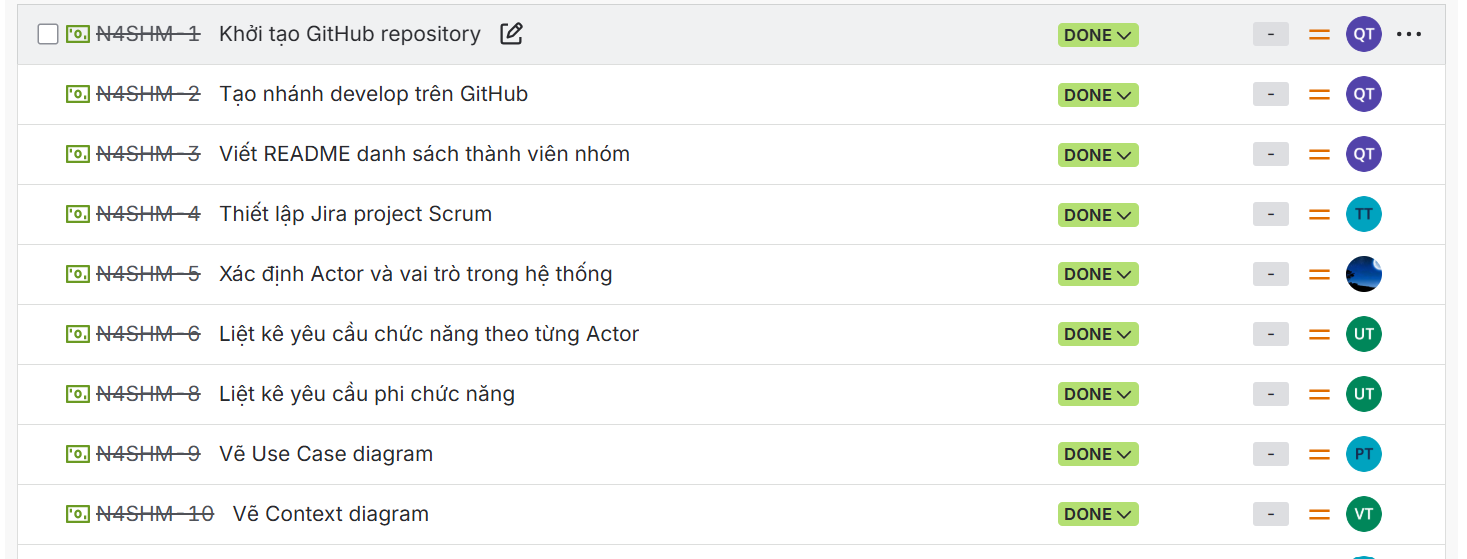
\includegraphics[width=\textwidth]{images/jira_initial_backlog.png}
    \caption{Các nhiệm vụ khởi tạo và phân tích yêu cầu trên Jira}
    \label{fig:jira-initial}
\end{figure}

\subsubsection{Luồng trạng thái công việc}

Mỗi nhiệm vụ được tạo dưới dạng một Jira issue với mã định danh duy nhất. Luồng xử lý được áp dụng như sau:

\begin{itemize}
    \item \textbf{To Do:} nhiệm vụ đã được xác định nhưng chưa bắt đầu hoặc đang chờ điều kiện thực hiện.
    \item \textbf{In Review:} kết quả đã hoàn thành bước đầu và đang được thành viên khác kiểm tra.
    \item \textbf{Done:} nhiệm vụ đáp ứng tiêu chí hoàn thành và đã được cập nhật vào sản phẩm hoặc báo cáo.
\end{itemize}

Một nhiệm vụ được xem là Done khi đáp ứng đầy đủ các điều kiện: nội dung hoặc mã nguồn đã hoàn thành, không còn lỗi nghiêm trọng được biết, đã được kiểm tra bởi ít nhất một thành viên khác và tài liệu liên quan đã được cập nhật.

\subsection{Quản lý chất lượng}

Mục tiêu quản lý chất lượng là bảo đảm hệ thống hoạt động đúng yêu cầu, dễ bảo trì và có tài liệu nhất quán. Nhóm áp dụng các biện pháp sau:

\subsubsection{Phòng ngừa lỗi}

\begin{itemize}
    \item Thống nhất cấu trúc thư mục Backend và Frontend trước khi phát triển chức năng.
    \item Sử dụng SQLAlchemy model và ràng buộc cơ sở dữ liệu để giảm dữ liệu trùng lặp.
    \item Băm mật khẩu bằng BCrypt và xác thực API bằng JWT.
    \item Xác thực dữ liệu đầu vào bằng Pydantic và HTTP exception tại Backend.
    \item Chia chức năng thành router riêng cho Authentication, Team và Submission.
\end{itemize}

\subsubsection{Review mã nguồn và tài liệu}

\begin{itemize}
    \item Thành viên phụ trách thực hiện tự kiểm tra trước khi cập nhật trạng thái In Review.
    \item Reviewer kiểm tra logic nghiệp vụ, định dạng response, lỗi truy cập dữ liệu và khả năng tích hợp với giao diện.
    \item Các chương báo cáo được viết bằng cùng một cấu trúc LaTeX và được tổng hợp trước khi nộp.
    \item Hình ảnh, bảng và sơ đồ phải có caption, label và được tham chiếu trong nội dung.
\end{itemize}

\subsubsection{Kiểm thử}

\begin{itemize}
    \item Kiểm thử RESTful API bằng cả Swagger UI và Postman.
    \item Kiểm thử trực tiếp các luồng người dùng trên trình duyệt Web.
    \item Kiểm tra dữ liệu trong SQLite sau các thao tác đăng ký, tạo đội, duyệt thành viên, quản lý thành viên và nộp bài.
    \item Thực hiện kiểm thử lại sau khi sửa lỗi đăng nhập, quản lý đội và quyền thao tác.
    \item Chạy Backend trên localhost bằng Uvicorn và sử dụng ngrok để hỗ trợ truy cập, tích hợp hoặc trình diễn từ bên ngoài máy phát triển.
\end{itemize}

\begin{table}[H]
    \centering
    \caption{Tiêu chí chất lượng của dự án}
    \label{tab:quality-criteria}
    \renewcommand{\arraystretch}{1.35}
    \begin{tabularx}{\textwidth}{|p{4cm}|p{4.2cm}|Y|}
        \hline
        \textbf{Nội dung} & \textbf{Tiêu chí} & \textbf{Phương pháp kiểm tra} \\
        \hline
        Chức năng lõi & Không có lỗi blocker trong các luồng đăng ký, đăng nhập, tạo đội, tham gia đội và nộp bài & Thực hiện test case và kiểm thử lại trên giao diện \\
        \hline
        API & Trả về đúng HTTP status code và JSON response & Swagger UI, Postman và Chrome DevTools \\
        \hline
        Dữ liệu & Không tạo dữ liệu đội hoặc bài nộp trùng trái quy tắc & Kiểm tra constraint và dữ liệu SQLite \\
        \hline
        Bảo mật cơ bản & Mật khẩu được băm, API bảo vệ yêu cầu JWT hợp lệ & Kiểm tra mã nguồn và request không có token \\
        \hline
        Tài liệu & Đánh số chương, hình, bảng và mục lục nhất quán & Biên dịch LaTeX và review chéo \\
        \hline
    \end{tabularx}
\end{table}

\subsection{Kế hoạch đào tạo và chia sẻ kiến thức}

Do thành viên đảm nhiệm các công việc khác nhau, nhóm tổ chức chia sẻ kiến thức ngắn theo nhu cầu của từng giai đoạn. Kế hoạch được trình bày trong Bảng \ref{tab:training-plan}.

\begin{table}[H]
    \centering
    \caption{Kế hoạch đào tạo và chia sẻ kiến thức}
    \label{tab:training-plan}
    \renewcommand{\arraystretch}{1.3}
    \begin{tabularx}{\textwidth}{|p{4.0cm}|p{3.2cm}|p{3.0cm}|Y|}
        \hline
        \textbf{Nội dung} & \textbf{Thành viên} & \textbf{Thời điểm} & \textbf{Tiêu chí miễn đào tạo} \\
        \hline
        Git, GitHub và quy trình nhánh \texttt{develop} & Toàn nhóm & Giai đoạn khởi tạo & Đã sử dụng Git và xử lý được merge conflict cơ bản \\
        \hline
        Jira Scrum và quản lý issue & Toàn nhóm & Giai đoạn khởi tạo & Tạo, phân công và cập nhật trạng thái issue thành thạo \\
        \hline
        FastAPI, SQLAlchemy và SQLite & Nhóm Backend & Trước khi hiện thực API & Đã xây dựng được CRUD API với SQLAlchemy \\
        \hline
        JWT, BCrypt và bảo vệ endpoint & Nhóm Backend & Trước module Authentication & Hiểu token, hash password và dependency injection \\
        \hline
        HTML, CSS, JavaScript và Fetch API & Nhóm Frontend & Trước giai đoạn tích hợp & Có thể gọi API và xử lý response trên giao diện \\
        \hline
        Draw.io, Figma và tài liệu thiết kế & Thành viên thiết kế & Giai đoạn thiết kế & Tạo được Use Case, ERD hoặc prototype theo quy ước nhóm \\
        \hline
        LaTeX và chuẩn hóa báo cáo & Toàn nhóm & Giai đoạn tài liệu & Biên dịch được file chương và xử lý lỗi hình, bảng, tham chiếu \\
        \hline
    \end{tabularx}
\end{table}

\section{Sản phẩm bàn giao}

Các sản phẩm bàn giao của dự án được tổ chức theo từng giai đoạn thay vì chỉ tập trung vào phiên bản cuối cùng. Điều này giúp nhóm có thể kiểm tra kết quả sớm và theo dõi mức độ hoàn thành trên Jira.

\begin{table}[H]
    \centering
    \caption{Danh sách sản phẩm bàn giao}
    \label{tab:project-deliverables}
    \renewcommand{\arraystretch}{1.35}
    \begin{tabularx}{\textwidth}{|p{1cm}|p{6.2cm}|p{3.1cm}|Y|}
        \hline
        \textbf{STT} & \textbf{Sản phẩm bàn giao} & \textbf{Giai đoạn} & \textbf{Ghi chú} \\
        \hline
        1 & GitHub repository, README, nhánh \texttt{develop} và cấu trúc thư mục & Khởi tạo & Nền tảng quản lý mã nguồn chung \\
        \hline
        2 & Jira project Scrum và danh sách issue N4SHM & Khởi tạo & Theo dõi phân công và trạng thái công việc \\
        \hline
        3 & Tài liệu yêu cầu: Actor, FR, NFR, Use Case và Context Diagram & Phân tích & Đầu vào cho SRS và thiết kế \\
        \hline
        4 & System Architecture, ERD, Data Design, API Design và Sequence Diagram & Thiết kế & Đầu vào cho hiện thực hệ thống \\
        \hline
        5 & Backend FastAPI và cơ sở dữ liệu SQLite & Hiện thực & Authentication, Team và Submission \\
        \hline
        6 & Giao diện Web cho đăng nhập, Dashboard và quản lý đội & Hiện thực & HTML, CSS và JavaScript \\
        \hline
        7 & Báo cáo kiểm thử và bằng chứng kết quả & Kiểm thử & Test case, kết quả PASS/FAIL và ảnh minh họa \\
        \hline
        8 & Bộ báo cáo bảy chương bằng LaTeX & Tài liệu hóa & Được tổng hợp và chuẩn hóa trước khi nộp \\
        \hline
        9 & Source code và hướng dẫn chạy hệ thống & Kết thúc & Phục vụ demo và đánh giá \\
        \hline
    \end{tabularx}
\end{table}

\section{Phân công trách nhiệm}

\subsection{Thành viên và vai trò chính}

\begin{table}[H]
    \centering
    \caption{Danh sách thành viên dự án}
    \label{tab:team-members}
    \renewcommand{\arraystretch}{1.35}
    \begin{tabularx}{\textwidth}{|p{1.1cm}|p{4.0cm}|p{3.2cm}|Y|}
        \hline
        \textbf{Mã} & \textbf{Họ và tên} & \textbf{MSSV} & \textbf{Vai trò chính} \\
        \hline
        QT & Lê Quang Trí & 042206005393 & Frontend Developer, tổng hợp và chuẩn hóa báo cáo \\
        \hline
        TT & Phạm Nguyễn Thanh Tùng & 075206019883 & Project Manager, Backend Developer \\
        \hline
        UT & Nguyễn Hà Thảo Uyên & 051306007680 & Backend Developer, phân tích yêu cầu, tác giả Chương 2 \\
        \hline
        VT & Trần Đặng Thảo Vân & 066306008936 & Backend Developer, thiết kế cơ sở dữ liệu và SDD \\
        \hline
        PT & Phạm Minh Tâm & 2251150033 & Frontend Developer, thiết kế giao diện và User Guide \\
        \hline
    \end{tabularx}
\end{table}

\subsection{Ma trận trách nhiệm RACI}

Ma trận RACI được sử dụng để làm rõ trách nhiệm trong từng nhóm công việc. Trong đó, \textbf{R} là người trực tiếp thực hiện, \textbf{A} là người chịu trách nhiệm cuối cùng, \textbf{C} là người được tham vấn và \textbf{I} là người được cập nhật thông tin.

\begin{table}[H]
    \centering
    \caption{Ma trận phân công trách nhiệm RACI}
    \label{tab:raci-matrix}
    \small
    \renewcommand{\arraystretch}{1.3}
    \resizebox{\textwidth}{!}{%
    \begin{tabular}{|p{7.2cm}|c|c|c|c|c|}
        \hline
        \textbf{Nhóm công việc} & \textbf{QT} & \textbf{TT} & \textbf{UT} & \textbf{VT} & \textbf{PT} \\
        \hline
        Lập kế hoạch và theo dõi dự án & C & A/R & C & I & I \\
        \hline
        GitHub repository và quản lý cấu trúc tài liệu & A/R & C & I & I & C \\
        \hline
        Phân tích yêu cầu chức năng và phi chức năng & C & A & R & C & R \\
        \hline
        Thiết kế giao diện và trải nghiệm người dùng & C & C & C & I & A/R \\
        \hline
        Thiết kế kiến trúc hệ thống và Backend & C & A/R & C & R & C \\
        \hline
        Thiết kế cơ sở dữ liệu và ERD & C & A & C & R & I \\
        \hline
        Hiện thực Authentication và Team API & R & A/R & R & R & I \\
        \hline
        Hiện thực Frontend và tích hợp API & R & C & C & I & A/R \\
        \hline
        Kiểm thử và sửa lỗi & C & A/R & R & C & R \\
        \hline
        Viết và chuẩn hóa báo cáo & A/R & C & R & R & R \\
        \hline
    \end{tabular}}
\end{table}

Hình \ref{fig:jira-report} thể hiện nhóm nhiệm vụ kiểm thử, viết các chương báo cáo và chuẩn hóa tài liệu cuối dự án. Trạng thái trên Jira cho phép Project Manager nhận biết phần việc đã hoàn thành, phần đang review và các nội dung còn chờ xử lý.

\begin{figure}[H]
    \centering
    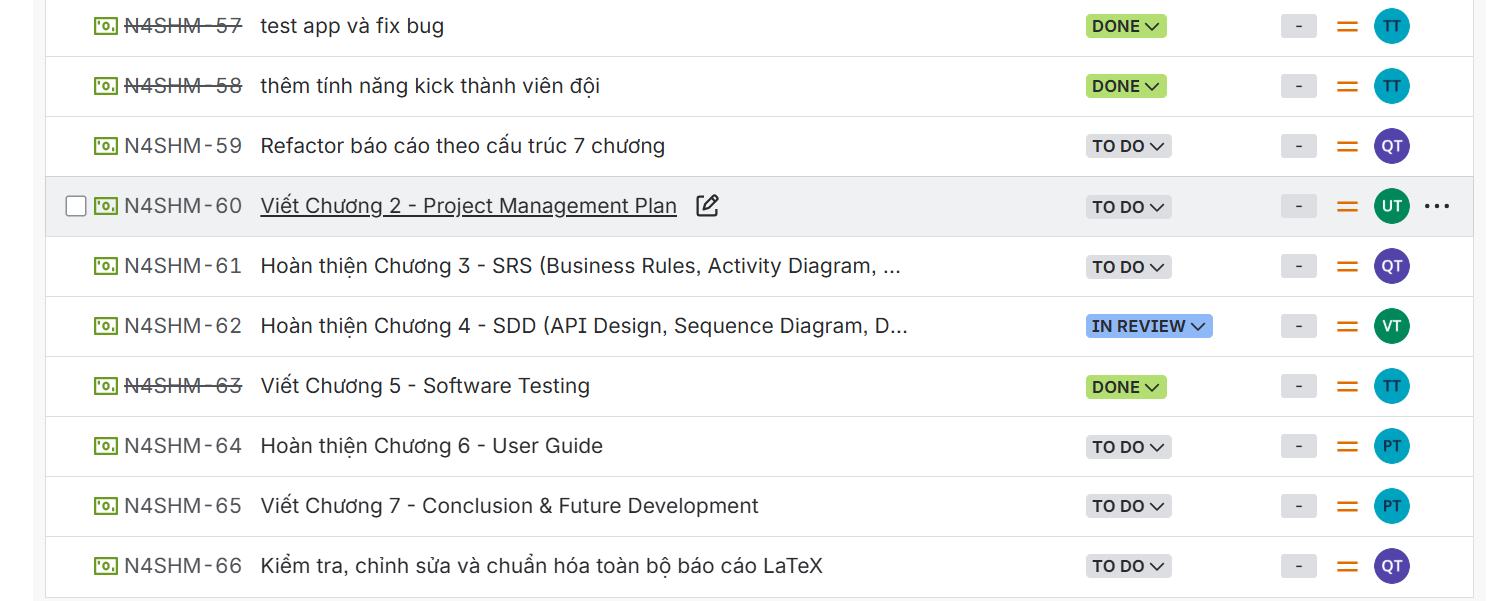
\includegraphics[width=\textwidth]{images/jira_report_and_closure.png}
    \caption{Các nhiệm vụ kiểm thử và hoàn thiện báo cáo trên Jira}
    \label{fig:jira-report}
\end{figure}

\section{Kế hoạch truyền thông}

Giao tiếp trong nhóm được tổ chức theo nguyên tắc ngắn gọn, có người chịu trách nhiệm và có kết quả được ghi nhận. Jira và GitHub là hai kênh chính để lưu lại bằng chứng công việc. Google Meet được sử dụng cho các buổi họp trực tuyến và demo chức năng; Zalo và Messenger được dùng để cập nhật nhanh, gửi tài liệu và xử lý vấn đề phát sinh; các buổi gặp trực tiếp được tổ chức khi cần thảo luận yêu cầu, tích hợp hệ thống, kiểm thử hoặc tổng hợp báo cáo.

\begin{table}[H]
    \centering
    \caption{Kế hoạch truyền thông của dự án}
    \label{tab:communication-plan}
    \renewcommand{\arraystretch}{1.3}
    \begin{tabularx}{\textwidth}{|p{3.0cm}|p{2.5cm}|p{4.0cm}|p{2.2cm}|Y|}
        \hline
        \textbf{Hoạt động} & \textbf{Đối tượng} & \textbf{Mục đích} & \textbf{Tần suất} & \textbf{Công cụ/Phương thức} \\
        \hline
        Lập kế hoạch Sprint & Toàn nhóm & Xác định công việc ưu tiên và người phụ trách cho tuần mới & Đầu mỗi Sprint & Jira, Google Meet hoặc gặp trực tiếp \\
        \hline
        Cập nhật tiến độ & Toàn nhóm & Báo cáo việc đã làm, việc tiếp theo và blocker & Trong Sprint và khi cần & Jira, Zalo, Messenger \\
        \hline
        Review chức năng & Developer và Reviewer & Kiểm tra logic, API, giao diện và dữ liệu trước khi xác nhận Done & Sau khi hoàn thành issue & Google Meet, Swagger UI, Postman, trình duyệt \\
        \hline
        Review tài liệu & Tác giả và người tổng hợp & Kiểm tra nội dung, hình, bảng, tham chiếu và định dạng & Khi hoàn thành chương & Gặp trực tiếp, Messenger/Zalo, LaTeX và GitHub \\
        \hline
        Xử lý lỗi khẩn cấp & Thành viên liên quan & Sửa lỗi ảnh hưởng luồng demo, API hoặc dữ liệu & Khi phát sinh & Zalo, Messenger, Google Meet và Jira issue \\
        \hline
        Tổng duyệt sản phẩm & Toàn nhóm & Kiểm tra luồng demo, báo cáo và gói nộp cuối & Cuối dự án & Gặp trực tiếp hoặc Google Meet \\
        \hline
    \end{tabularx}
\end{table}

Các quyết định quan trọng như thay đổi chức năng, thay đổi cấu trúc dữ liệu hoặc thay đổi định dạng báo cáo phải được ghi nhận trong Jira issue hoặc commit để tránh thất lạc thông tin.

\section{Quản lý cấu hình}

\subsection{Quản lý tài liệu}

Tài liệu dự án được tổ chức trong khu vực báo cáo LaTeX của repository. Mỗi chương được viết thành file riêng để các thành viên có thể làm việc độc lập và giảm xung đột chỉnh sửa. Quy ước quản lý tài liệu gồm:

\begin{itemize}
    \item Tên file chương sử dụng dạng \texttt{ChapterN.tex}.
    \item Mỗi chương có file \texttt{test\_ChapterN.tex} để biên dịch và kiểm tra độc lập.
    \item Hình ảnh được đặt trong thư mục \texttt{images} và đặt tên bằng chữ thường, không dấu.
    \item Tất cả bảng và hình phải có \texttt{caption}, \texttt{label} và tham chiếu bằng \texttt{ref}.
    \item Thành viên tổng hợp kiểm tra mục lục, đánh số chương và lỗi biên dịch trước khi merge.
    \item Phiên bản quan trọng được lưu trong lịch sử Git thay vì tạo nhiều bản sao không kiểm soát.
\end{itemize}

\subsection{Quản lý mã nguồn}

Mã nguồn được lưu trên GitHub. Dựa trên kế hoạch Jira, nhóm đã khởi tạo repository và tạo nhánh \texttt{develop}. Chiến lược quản lý mã nguồn được áp dụng như sau:

\begin{itemize}
    \item \texttt{main}: chứa phiên bản ổn định dùng để demo hoặc nộp sản phẩm.
    \item \texttt{develop}: chứa phiên bản tích hợp của nhóm trong quá trình phát triển.
    \item Nhánh theo nhiệm vụ: được tạo khi thành viên thực hiện chức năng hoặc sửa lỗi riêng.
    \item Mỗi commit cần mô tả rõ chức năng hoặc Jira issue, ví dụ \texttt{N4SHM-58 add kick member feature}.
    \item Không đưa thư mục môi trường ảo, file cache hoặc thông tin bí mật lên repository.
    \item Trước khi merge, thành viên phải cập nhật code mới nhất, tự kiểm thử và xử lý conflict.
\end{itemize}

Đối với cấu hình bảo mật, các giá trị như JWT SECRET KEY cần được chuyển sang file môi trường và đưa file này vào \texttt{.gitignore}. Cách làm này giúp giảm nguy cơ lộ thông tin nhạy cảm khi chia sẻ mã nguồn.

Tại thời điểm ghi nhận báo cáo, repository công khai có tên \textbf{SEAL-Hackathon-Management}, được tổ chức thành các khu vực như \texttt{backend}, \texttt{src}, \texttt{docs} và \texttt{report-latex}. Giao diện GitHub hiển thị hai nhánh và 97 commit. Các số liệu này chỉ phản ánh trạng thái repository tại thời điểm chụp; nhóm không sử dụng số lượng commit làm tiêu chí duy nhất để đánh giá mức độ đóng góp của thành viên.

\begin{figure}[H]
    \centering
    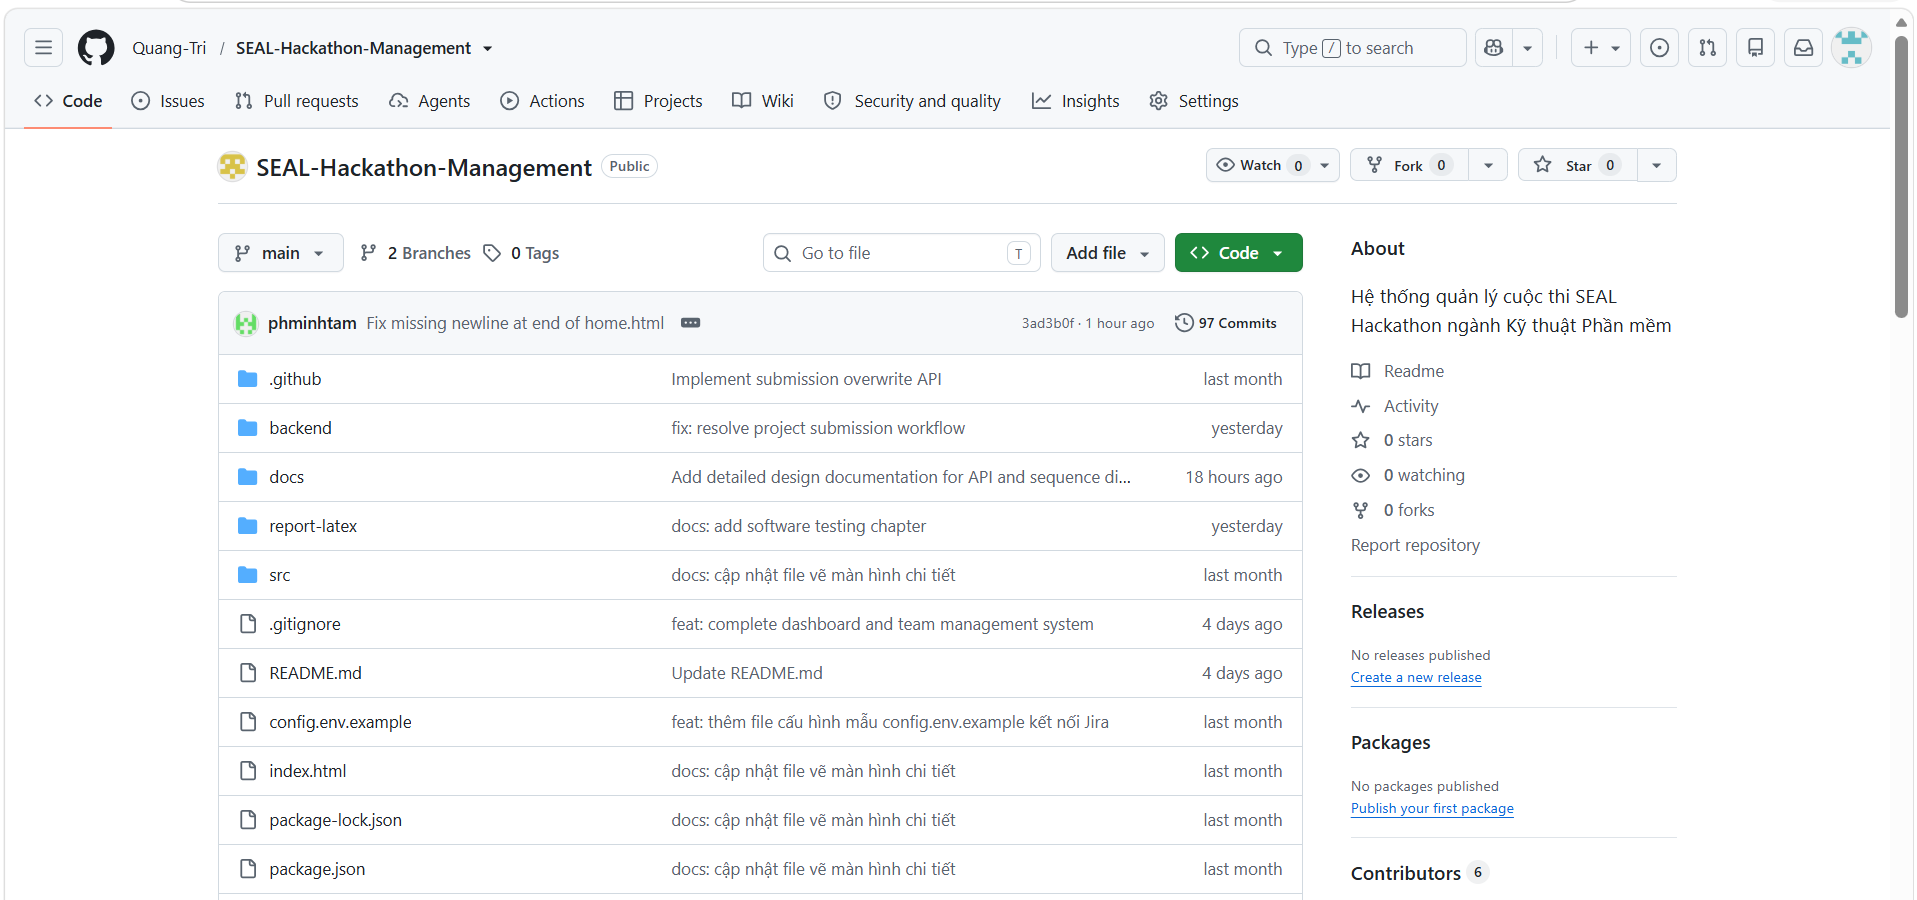
\includegraphics[width=\textwidth]{images/github_repository_overview.png}
    \caption{Trang chính GitHub repository của dự án}
    \label{fig:github-repository-overview}
\end{figure}

\begin{figure}[H]
    \centering
    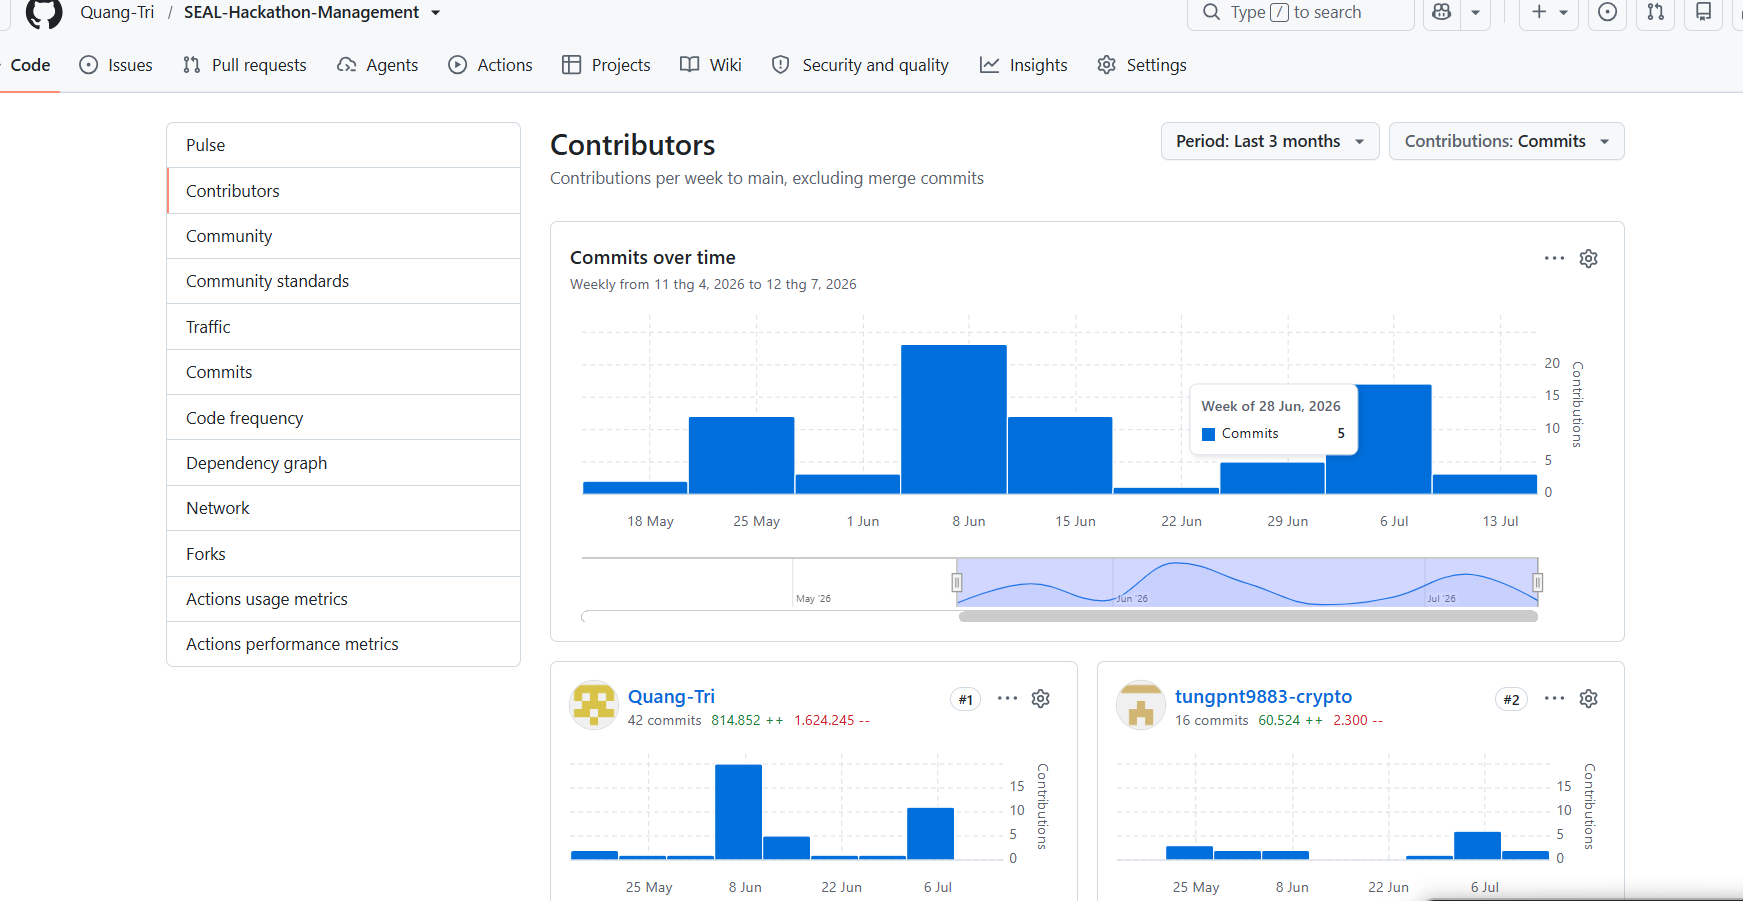
\includegraphics[width=\textwidth]{images/github_contribution_history.png}
    \caption{Lịch sử commit và hoạt động đóng góp trên GitHub}
    \label{fig:github-contribution-history}
\end{figure}

\subsection{Công cụ và hạ tầng}

\begin{table}[H]
    \centering
    \caption{Công cụ và công nghệ của dự án}
    \label{tab:tools-infrastructure}
    \renewcommand{\arraystretch}{1.3}
    \begin{tabularx}{\textwidth}{|p{4.0cm}|Y|}
        \hline
        \textbf{Nhóm công cụ} & \textbf{Công cụ/Công nghệ} \\
        \hline
        Backend & Python, FastAPI 0.139.0, Uvicorn 0.51.0 \\
        \hline
        Cơ sở dữ liệu & SQLite 3, SQLAlchemy 2.0.51 \\
        \hline
        Xác thực và bảo mật & python-jose 3.3.0, Passlib 1.7.4, BCrypt 4.0.1, JWT \\
        \hline
        Kiểm tra dữ liệu & Pydantic 2.13.4, python-multipart 0.0.9 \\
        \hline
        Frontend & HTML5, CSS3, JavaScript \\
        \hline
        Môi trường phát triển & Localhost, Uvicorn và trình duyệt Web \\
        \hline
        Quản lý mã nguồn & Git và GitHub \\
        \hline
        Quản lý dự án & Jira Scrum với Sprint một tuần \\
        \hline
        Thiết kế & Figma, Draw.io \\
        \hline
        Kiểm thử & Swagger UI, Postman, trình duyệt Web và kiểm tra dữ liệu SQLite \\
        \hline
        Tài liệu và giao tiếp & LaTeX, Google Meet, Zalo, Messenger và gặp trực tiếp \\
        \hline
        Chạy và chia sẻ thử nghiệm & Uvicorn trên localhost và ngrok (pyngrok 7.1.6) \\
        \hline
    \end{tabularx}
\end{table}

\section{Kết luận chương}

Chương 2 đã trình bày kế hoạch quản lý dự án của \textbf{SEAL Hackathon Management System}, bao gồm phạm vi, WBS không sử dụng man-day, mục tiêu, rủi ro, lịch tám Sprint một tuần, quản lý chất lượng, kế hoạch đào tạo, sản phẩm bàn giao, ma trận trách nhiệm, kế hoạch truyền thông và quản lý cấu hình.

Việc sử dụng Jira giúp nhóm phân chia và theo dõi các nhiệm vụ một cách minh bạch, trong khi GitHub hỗ trợ kiểm soát phiên bản mã nguồn và tài liệu. Kế hoạch này tạo cơ sở để nhóm phối hợp giữa Frontend, Backend, phân tích, kiểm thử và viết báo cáo, đồng thời giúp kiểm soát các giới hạn của phiên bản hiện tại như phân quyền Admin/Judge và lưu dữ liệu chấm điểm.

Các yêu cầu chức năng, phi chức năng và quy tắc nghiệp vụ của hệ thống sẽ được trình bày chi tiết hơn trong Chương 3 -- Software Requirements Specification.
